\section{O (suposto) Problema}

\begin{frame}{Teólogos que veem problema}
 \begin{columns}
  \begin{column}{0.7\textwidth}
   \begin{itemize}
    \item<2->[$\bullet$] \textcolor{NordBrightCyan}{\textbf{Gilkey}}: teólogos não acreditam que Deus 
    tenha realizado milagres!
     \begin{itemize}
      \item<5-> a Bíblia é um livro de interpretação
      \item<6-> dizer $\times$ crer
     \end{itemize}
    \item<3->[$\bullet$] \textcolor{NordBrightCyan}{\textbf{Bultmann}}: Deus não age no mundo!
     \begin{itemize}
      \item<7-> a história é uma \textcolor{NordYellow}{sequência fechada de efeitos}.
      \item<8-> não pode sofrer intervenções de poderes sobrenaturais
      \item<9-> causa e efeito
      \item<10-> Lei dos Medos e Persas
     \end{itemize}
    \item<4->[$\bullet$] \textcolor{NordBrightCyan}{\textbf{Macquarrie}}: rompimento da ordem natural
     \begin{itemize}
      \item<11-> ciência e história são \textbf{\textcolor{NordRed}{inconciliáveis}}
      com a ideia de ``milagres''.
      \item<12-> motivo: causa e efeito
       \begin{itemize}
        \item<13->[-] conhecimento limitado apenas temporariamente.
       \end{itemize}
     \end{itemize}
   \end{itemize}
  \end{column}
  \begin{column}{0.3\textwidth}
   \only<2, 5-6>{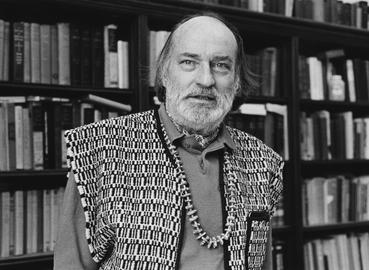
\includegraphics[width = 4cm]{gilkey}}
   \only<3, 7-10>{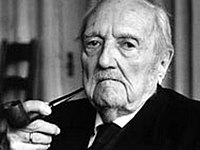
\includegraphics[width = 4cm]{bultmann}}
   \only<4, 11-13>{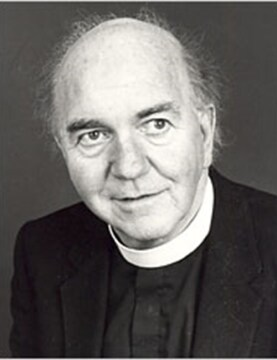
\includegraphics[width = 4cm]{macquarrie}}
  \end{column}
 \end{columns}
\end{frame}

\begin{frame}{Teólogos que veem problema}
 \centering
 \begin{minipage}{\textwidth}
  \begin{exampleblock}{\textbf{Observações}}
   \begin{itemize}
    \item<2->[$\bullet$] Bultmann e Macquarrie acham compatíveis a ``ação geral'' de
     Deus (preservação da existência do mundo), mas não a ``ação particular'';
    \item<3->[$\bullet$] A ação particular é um problema porque: é incompatível
     com a ciência moderna.
     \begin{itemize}
      \item<4-> a ciência \textcolor{NordYellow}{demonstra} ou 
       \textcolor{NordYellow}{pressupõe} que Deus não age assim;
      \item<5-> a ciência é a Razão.
     \end{itemize}
   \end{itemize}
  \end{exampleblock} 
 \end{minipage}
\end{frame}

\begin{frame}{Filósofo ou Cientistas que veem problema}
 \begin{columns}
  \begin{column}{0.45\textwidth}
   \begin{itemize}
    \justifying
    \item<2-3,8-14>[$\bullet$] \textcolor{NordBrightCyan}{Philip Clayton}: a ciência 
     tem a capacidade de explicar e prever os fenômenos naturais.
   \end{itemize}
   \vspace{0.5cm}
   \centering
   \only<2-3, 8-14>{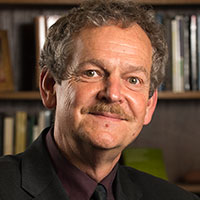
\includegraphics[width = 4cm]{clayton}}
   \only<4>{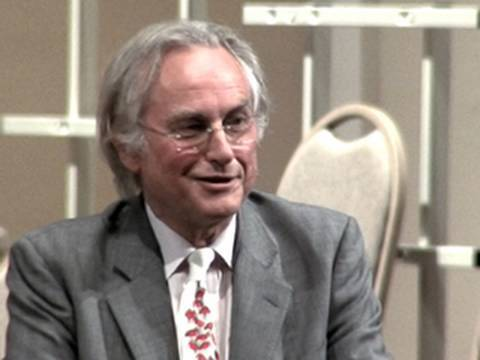
\includegraphics[width = 4cm]{dawkins}}
   \only<5>{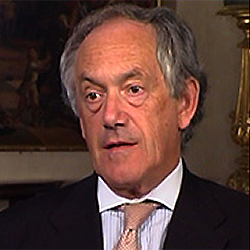
\includegraphics[width = 4cm]{peter}}
   \only<7>{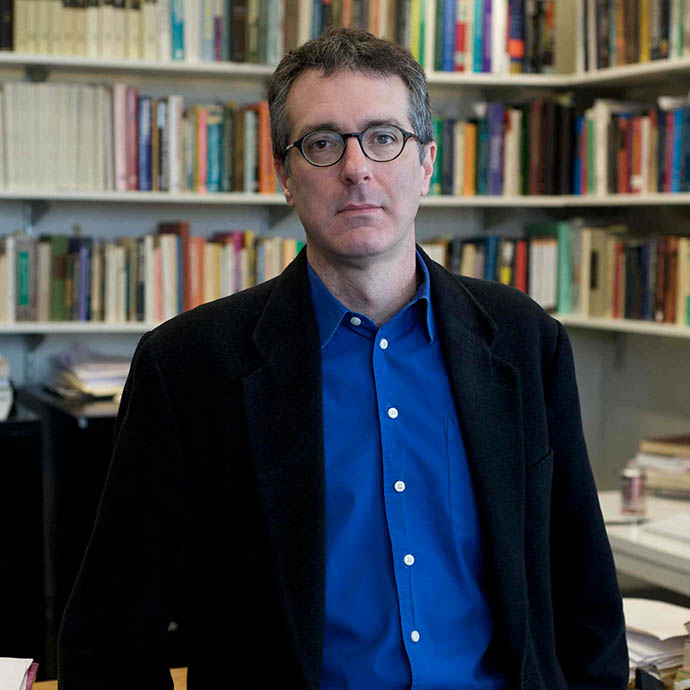
\includegraphics[width = 4cm]{orr}}
   \only<6>{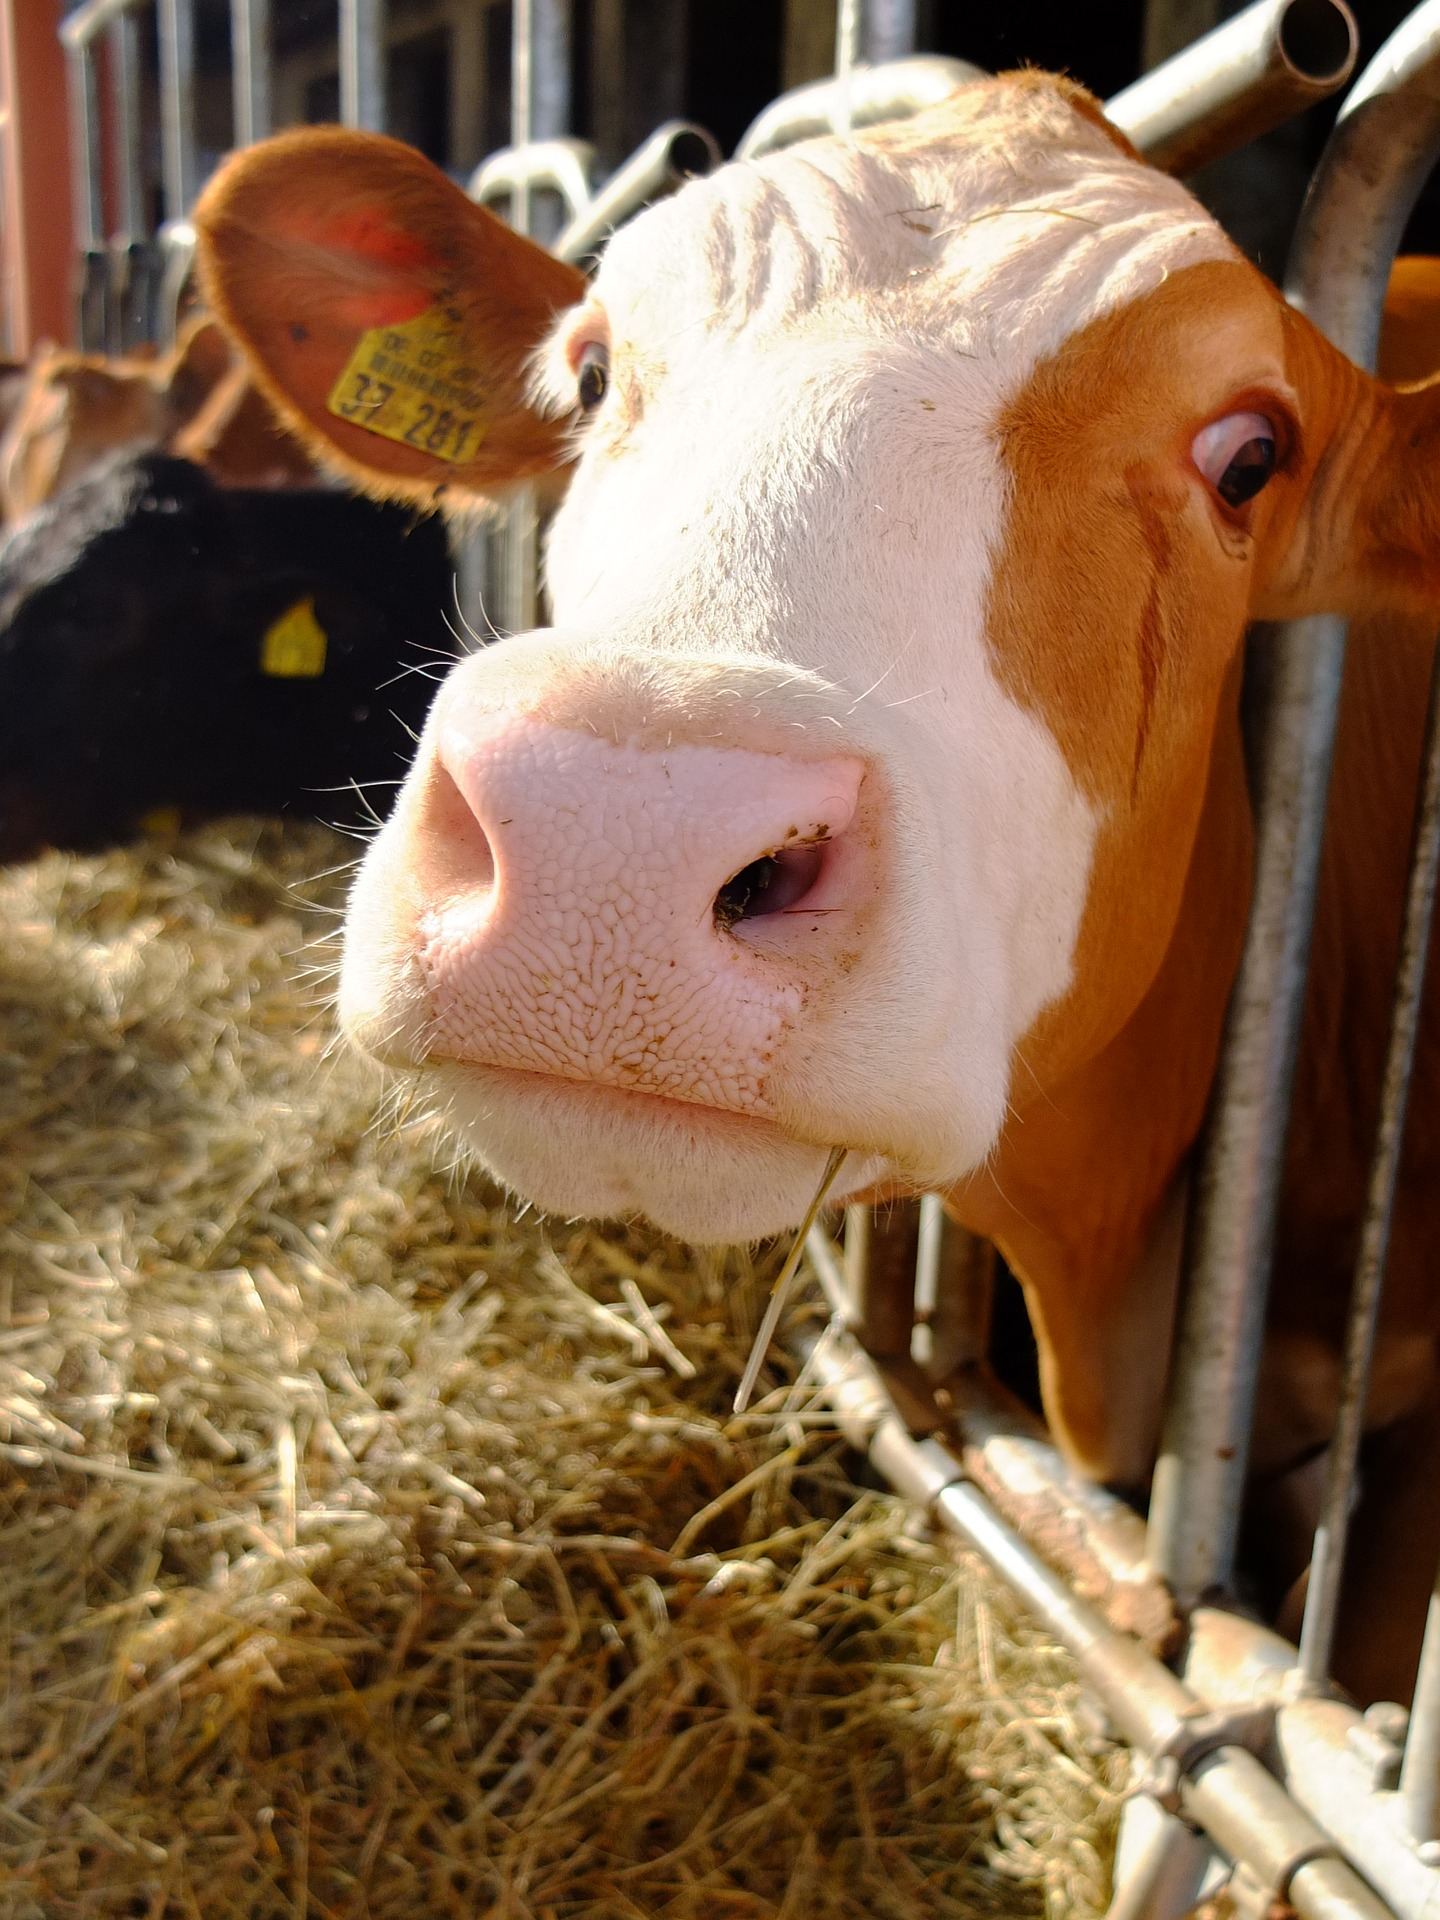
\includegraphics[width = 4cm]{vaca}}
   \only<15>{
\includegraphics[width = 4cm]{merovingian}}
   \only<16>{
\includegraphics[width = 4cm]{sherlock}}
   \only<17>{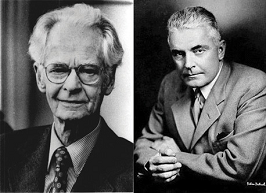
\includegraphics[width = 4cm]{watson-skinner}}
  \end{column}
  \begin{column}{0.55\textwidth}
   \begin{itemize}
    \item<3-> Cientitas com Clayton: 
     \begin{itemize}
      \item<4-> \onslide<4->{Richard Dawkins}\onslide<5->{, Peter Atkins} \onslide<6->{(loucos?)}
      \item<7-> H. Allen Orr (sensato)
     \end{itemize}
    \item<8-|alert@8> Ciência $\Longleftrightarrow$ \textcolor{NordYellow}{Determinismo}
     \begin{itemize}
      \item<9-> Exclusão de Deus (ação particular)
      \item<10-> At 17.18: estóicos \textit{vs} epicureus
       \begin{itemize}
        \item<11-> virtude: reação diante do determinismo materialista
        \item<12-> o ser humano não pode determinar seu destino
        \item<13-> ataraxia
        \item<14-> Síndrome de Gabriela
       \end{itemize}
      \item<15-> Filme Matrix
      \item<16-> Sherlock Holmes
      \item<17-> Skinner e Watson
     \end{itemize}
   \end{itemize}
  \end{column}
 \end{columns}
\end{frame}

\begin{frame}{Um dos Perigos do Determinismo}
 \begin{quote}
  \onslide<2->{
   Nossos membros estão praticamente sempre fazendo o que 
   \textcolor{NordOrange}{querem} fazer --- o que eles 
   \textcolor{NordOrange}{escolhem} fazer --- mas nós cuidamos para que eles 
   queiram fazer precisamente as coisas	que são melhores para eles e para a 
   comunidade.
  }
  \onslide<3->{Seu comportamento é determinado, ainda que eles sejam livres.}
  \onslide<4->{Ditadura e liberdade, determinismo e livre-arbítrio.}
  \onslide<5->{O que é isso senão pseudoquestões de origem linguística?}
  \onslide<6->{Quando perguntamos o que o Homem pode fazer do Homem, nós não 
  queremos dizer	a mesma coisa por ``homem'' em ambos os casos.}
  \onslide<7->{Queremos perguntar o que alguns poucos homens podem fazer da 
  humanidade.}
  \onslide<8->{E essa é a questão central do século XX.} 
  \onslide<9->{Que tipo de mundo podemos construir --- nós que entendemos a 
  ciência do comportamento?} \onslide<10->{(\textcolor{NordYellow}{Skinner})}
 \end{quote}
\end{frame}

\begin{frame}{\textbf{Resumo do Problema}}
 \centering
 \begin{minipage}{\textwidth}
  \begin{exampleblock}{\textbf{Resumo do ``Problema''}}
   \begin{enumerate}[(1)]
    \item<2-> A Ciência propõe e valida Leis Naturais;
    \item<3-> As ações particulares de Deus violariam as Leis Naturais;
    \item<4-> Isso é incompatível com a Ciência.
   \end{enumerate}
  \end{exampleblock}
 \end{minipage}
\end{frame}
